\section{Inverting Amplifier}

\subsection{Pengantar Inverting Amplifier}
\begin{frame}{Pengantar Inverting Amplifier}
	\begin{itemize}
		\item Inverting amplifier: rangkaian op amp paling dasar.
		\item Menggunakan negative feedback untuk menstabilkan keseluruhan voltage gain.
		\item Keseluruhan voltage gain perlu distabilkan karena $ A_{VOL} $ sangat besar dan tidak stabil untuk digunakan tanpa feedback.
		\item Contohnya, 741C memiliki $ A_{VOL} $ minimum sebesar 20.000 dan $ A_{VOL} $ maksimum lebih dari 200.000.
		\item Voltage gain yang tidak dapat dipredisksi dari magnitude dan variasi ini tidak berguna tanpa feedback.
	\end{itemize}
\end{frame}

\subsection{Inverting Negative Feedback}
\begin{frame}{Inverting Negative Feedback}
	\begin{figure}
		\centering
		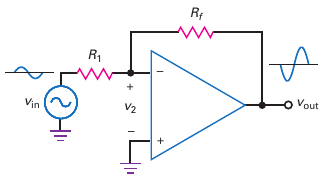
\includegraphics[height=0.5\textheight]{gambar/fig-16.12}
		\caption{Inverting amplifier}
		\label{fig-16.12}
	\end{figure}
\end{frame}

\begin{frame}{Inverting Negative Feedback}
	\begin{itemize}
		\item Gambar \ref{fig-16.12} menunjukkan sebuah inverting amplifier.
		\item Tegangan power-supply tidak ditampilkan agar gambar lebih sederhana.
		\item Tegangan input $ v_{in} $ men-drive inverting input melalui resistor $ R_1 $.
		\item Menghasilkan tegangan inverting output $ v_2 $.
		\item Tegangan input dikuatkan oleh open-loop voltage gain untuk menghasilkan tegangan inverted output.
		\item Tegangan output diumpanbalik ke input melalui resistor feedback $ R_f $.
		\item Menghasilkan negative feedback karena output memiliki beda fasa sebesar 180$ ^\circ $ dengan input.
		\item Dengan kata lain, setiap perubahan di $ v_2 $ yang dihasilkan oleh tegangan input berkebalikan dengan sinyal output.
	\end{itemize}
\end{frame}

\begin{frame}{Inverting Negative Feedback}
	\begin{itemize}
		\item Bagaimana negative feedback dapat menstabilkan overall voltage gain?
		\item Jika open-loop voltage gain $ A_{VOL} $ meningkat dengan alasan apa pun, tegangan output akan meningkat dan memberikan tegangan feedback yang lebih banyak ke inverting input.
		\item Tegangan feedback yang berkebalikan ini akan mereduksi tegangan $ v_2 $.
		\item Karena itu, meskipun $ A_{VOL} $ meningkat,$ v_2 $ menurun, dan output akhir meningkat jauh lebih sedikit daripada tanpa negative feedback.
	\end{itemize}
\end{frame}

\subsection{Virtual Ground}
\begin{frame}{Virtual Ground}
	\begin{multicols}{2}
		\begin{figure}
			\centering
			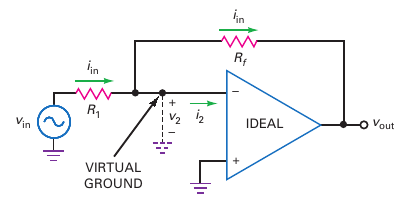
\includegraphics[height=0.4\textheight]{gambar/fig-16.13}
			\caption{Konsep virtual ground}
			\label{fig-16.13}
		\end{figure}
	\columnbreak
		\begin{itemize}
			\item Analisis inverting amplifier lebih mudah
			\item Berdasarkan op amp ideal:
			\begin{itemize}
				\item $ R_{in} = \infty \rightarrow i_2 = 0$
				\item $ A_{VOL} = \infty \rightarrow v_2 = 0 \rightarrow $
			\end{itemize}
			\item Karena $ i_2 = 0 $ maka $ i_{R_f} = i_{in} $
		\end{itemize}
	\end{multicols}
\end{frame}

\subsection{Voltage Gain \& Impedansi Input}
\begin{frame}{Voltage Gain \& Impedansi Input}
	\begin{multicols}{2}
		\begin{figure}
			\centering
			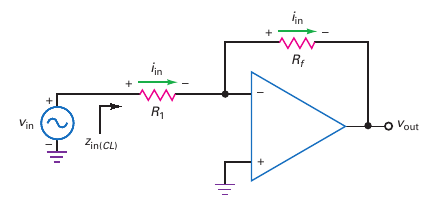
\includegraphics[height=0.4\textheight]{gambar/fig-16.14}
			\caption{Inverting amplifier memiliki arus yang sama yang melewati kedua resistor}
			\label{fig-16.14}
		\end{figure}
	\columnbreak
		\begin{itemize}
			\item Tegangan input: $ v_{in} = i_{in} R_1 $
			\item Tegangan output: $ v_{out} = -i_{in} R_f $
			\item Penguatan tegangan closed-loop:
			\begin{equation}\label{pers.16.3}
				A_{v(CL)} = \frac{-R_f}{R_1}
			\end{equation}
			%\item $ A_{v(CL)} < A_{VOL} $
			\item Impedansi input:
			\begin{equation}\label{pers.16.4}
				z_{in(CL)} = R_1
			\end{equation}
		\end{itemize}
	\end{multicols}
\end{frame}

\subsection{Bandwidth}
\begin{frame}{Bandwidth}
	\begin{multicols}{2}
		\begin{figure}
			\centering
			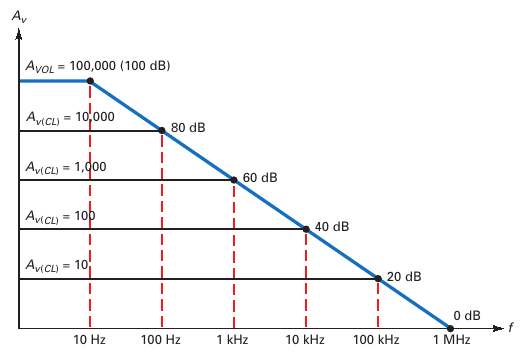
\includegraphics[height=0.6\textheight]{gambar/fig-16.15}
			\caption{Voltage gain yang lebih kecil menghasilkan bandwidth yang lebih besar}
			\label{fig-16.15}
		\end{figure}
	\columnbreak
		\begin{itemize}
			\item Closed-loop bandwidth:
			\begin{equation}\label{pers.16.5}
				f_{2(CL)} = \frac{f_{unity}}{A_{v(CL)}}
			\end{equation}
			\item Gain-band-width product (GBW):
			\begin{equation}\label{pers.16.6}
				f_{unity} = A_{v(CL)}f_{2(CL)}
			\end{equation}
		\end{itemize}
	\end{multicols}
\end{frame}

\subsection{Bias dan Offset}
\begin{frame}{Bias dan Offset}
	\begin{itemize}
		\item Total error tegangan output:
		\begin{equation}\label{pers.16.7}
			V_{error} \cong \pm A_{v(CL)} (\pm V_{1err} \pm V_{2err} \pm V_{3err} )
		\end{equation}
		\item Error tegangan input:
		\begin{equation}\label{pers.16.8}
			V_{1err} = (R_{B1} - R_{(B2)}) I_{in(bias)}
		\end{equation}
		\begin{equation}\label{pers.16.9}
			V_{2err} = (R_{B1} + R_{(B2)}) \frac{I_{in(off)}}{2}
		\end{equation}
		\begin{equation}\label{pers.16.10}
			V_{3err} = V_{in(off)}
		\end{equation}
		\item Resistor Thevenin
		\begin{equation}\label{pers.16.11}
			R_{B2} = R_1 \parallel R_f
		\end{equation}
	\end{itemize}
\end{frame}

\subsection{Contoh Soal 2.7}
\begin{frame}{Contoh Soal 2.7}
	\begin{multicols}{2}
		\begin{center}
			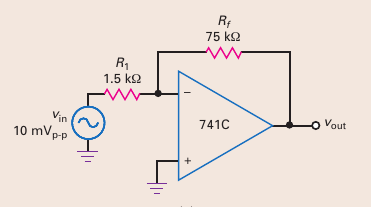
\includegraphics[width=\linewidth]{gambar/fig-16.16a}
		\end{center}
		\columnbreak
		\begin{itemize}
			\item Pertanyaan:
			\begin{itemize}
				\item Berapa penguatan tegangan closed-loop dan bandwidth closed-loop nya?
				\item Berapa tegangan output di 1 kHz? dan di 1 MHz?
			\end{itemize}
		\end{itemize}
	\end{multicols}
\end{frame}

\begin{frame}{Contoh Soal 2.7}
	\begin{multicols}{2}
		\begin{center}
			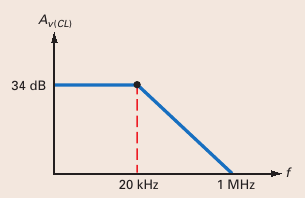
\includegraphics[width=\linewidth]{gambar/fig-16.16b}
		\end{center}
		\columnbreak
		\begin{itemize}
			\item Jawaban:
			\begin{itemize}
				\item Penguatan tegangan closed-loop:
				\[ A_{v(CL)} = \frac{-R_f}{R_1} = \frac{-75 \text{ k}\Omega}{1.5 \text{ k}\Omega} = -50\]
				\item Bandwidth closed-loop:
				\[ f_{2(CL)} = \frac{f_{unity}}{A_{v(CL)}} = \frac{1 \text{ MHz}}{50} = 20 \text{ kHz}\]
				\item Ideal bode-plot dari $ A_{v(CL)} $
			\end{itemize}
		\end{itemize}
	\end{multicols}
\end{frame}

\begin{frame}{Contoh Soal 2.7}
	\begin{multicols}{2}
		\begin{center}
			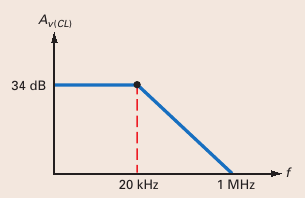
\includegraphics[width=\linewidth]{gambar/fig-16.16b}
		\end{center}
		\columnbreak
		\begin{itemize}
			\item Jawaban:
			\begin{itemize}
				\item Tegangan output di 1 kHz:
				\begin{align*}
					v_{out} &= (A_{v(CL)})(v_{in}) = (-50)(10 \text{ mVp-p}) \\
					&= -500 \text{ mVp-p}
				\end{align*}
				\item Tegangan output di 1 MHz. Karena 1 MHz adalah unity-gain frekuensinya, maka
					\[ v_{out} = -10 \text{ mVp-p} \]
				\item Tanda negatif menunjukkan phase-shift $ 180^{\circ} $ antara input dan output
			\end{itemize}
		\end{itemize}
	\end{multicols}
\end{frame}

\subsection{Latihan Soal 2.7}
\begin{frame}{Latihan Soal 2.7}
	\begin{multicols}{2}
		\begin{center}
			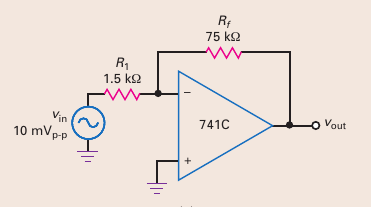
\includegraphics[width=\linewidth]{gambar/fig-16.16a}
		\end{center}
		\columnbreak
		\begin{itemize}
			\item Pertanyaan:
			\begin{itemize}
				\item Berapa tegangan output di 100 kHz ?
				\item \textit{Hint:} Gunakan persamaan \[ A_v = \frac{A_{v(mid)}}{ \sqrt{1 + (f/f_2)^2} } \]
			\end{itemize}
		\end{itemize}
	\end{multicols}
\end{frame}

\subsection{Contoh Soal 2.8}
\begin{frame}{Contoh Soal 2.8}
	\begin{multicols}{2}
		\begin{center}
			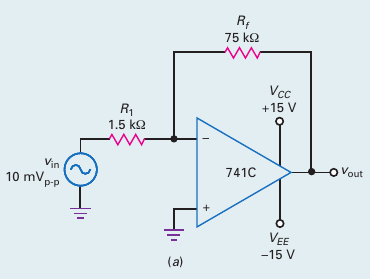
\includegraphics[width=\linewidth]{gambar/fig-16.17a}
		\end{center}
		\columnbreak
		\begin{itemize}
			\item Pertanyaan:
			\begin{itemize}
				\item Berapa tegangan output ketika $ v_{in} = 0 $?
			\end{itemize}
		\end{itemize}
	\end{multicols}
\end{frame}

\begin{frame}{Contoh Soal 2.8}
	\begin{multicols}{2}
		\begin{center}
			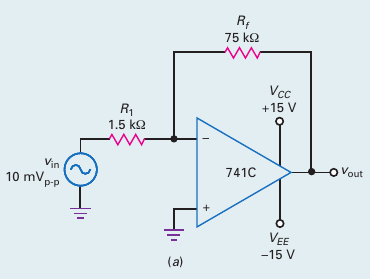
\includegraphics[width=\linewidth]{gambar/fig-16.17a}
		\end{center}
		\columnbreak
		\begin{itemize}
			\item Jawaban:
			\begin{itemize}
				\item Berdasarkan Tabel di Gambar \ref{tab-16.01}, didapatkan:
				\[ I_{\text{in}(\text{bias})} = 80 \text{ nA} \]
				\[ I_{\text{in}(\text{off})} = 20 \text{ nA} \]
				\[ V_{\text{in}(\text{off})} = 2 \text{ mV} \]
				\item Berdasarkan Persamaan \ref{pers.16.11}:
				\begin{align*}
					R_{B2} &= R_1 \parallel R_f = 1.5 \text{ k}\Omega \parallel 75 \text{ k}\Omega \\
					&= 1.47 \text{ k}\Omega
				\end{align*}
			\end{itemize}
		\end{itemize}
	\end{multicols}
\end{frame}

\begin{frame}{Contoh Soal 2.8}
	\begin{multicols}{2}
		\begin{center}
			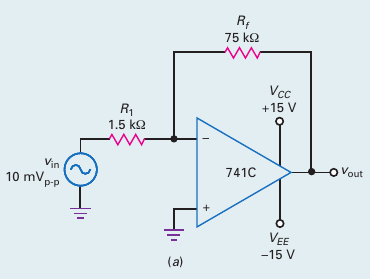
\includegraphics[width=\linewidth]{gambar/fig-16.17a}
		\end{center}
		\columnbreak
		\begin{itemize}
			\item Jawaban:
			\begin{itemize}
				\item Error tegangan input:
				\begin{align*}
					V_{1err} &= (R_{B1} - R_{B2})I_{in(bias)} \\
					&= ( - 1.47 \text{ k}\Omega )(80 \text{ nA}) \\
					&= -0.118 \text{ mV} \\
					V_{2err} &= (R_{B1} + R_{B2}) \frac{I_{in(off)}}{2} \\
					&= ( 1.47 \text{ k}\Omega )(10 \text{ nA}) \\
					&= 0.0147 \text{ mV} \\
					V_{3err} &= V_{in(off)} = 2 \text{ mV}
				\end{align*}
			\end{itemize}
		\end{itemize}
	\end{multicols}
\end{frame}

\begin{frame}{Contoh Soal 2.8}
	\begin{multicols}{2}
		\begin{center}
			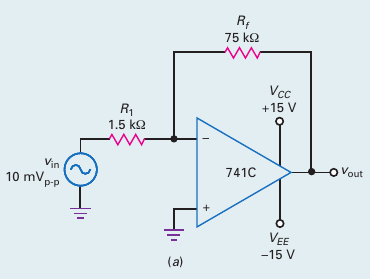
\includegraphics[width=\linewidth]{gambar/fig-16.17a}
		\end{center}
		\columnbreak
		\begin{itemize}
			\item Jawaban:
			\begin{itemize}
				\item Penguatan tegangan closed-loop:
				\[ A_{v(CL)} = \frac{-R_f}{R_1} = \frac{-75 \text{ k}\Omega}{1.5 \text{ k}\Omega} = -50\]
				\item Error tegangan output:
				\begin{align*}
					V_{error} &= \pm 50 (V_{1err} + V_{2err} + V_{2err}) \\
					&= \pm 50 (0.118 \text{mV} + 0.0147 \text{mV} + 2 \text{mV}) \\
					&= \pm 107 \text{ mV}
				\end{align*}
			\end{itemize}
		\end{itemize}
	\end{multicols}
\end{frame}

\subsection{Latihan Soal 2.8}
\begin{frame}{Latihan Soal 2.8}
	\begin{multicols}{2}
		\begin{center}
			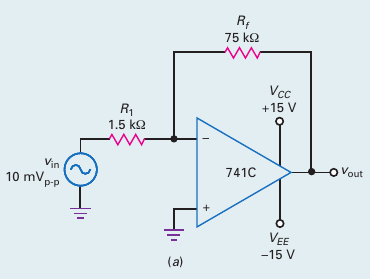
\includegraphics[width=\linewidth]{gambar/fig-16.17a}
		\end{center}
		\columnbreak
		\begin{itemize}
			\item Pertanyaan:
			\begin{itemize}
				\item Jika op amp yang digunakan adalah LF157A, berapa tegangan output ketika $ v_{in} = 0 $?
			\end{itemize}
		\end{itemize}
	\end{multicols}
\end{frame}

\subsection{Contoh Soal 2.9}
\begin{frame}{Contoh Soal 2.9}
	\begin{multicols}{2}
		\begin{center}
			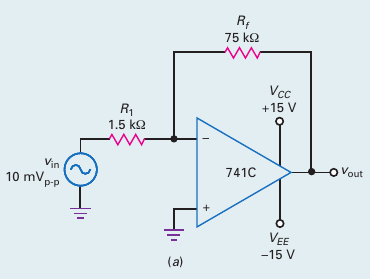
\includegraphics[width=\linewidth]{gambar/fig-16.17a}
		\end{center}
		\columnbreak
		\begin{itemize}
			\item Pertanyaan:
			\begin{itemize}
				\item Diketahui: \\
				$ I_{in(bias)} = 500 \text{ nA} $, \\
				$ I_{in(off)} = 200 \text{ nA}$, dan \\
				$ V_{in(off)} = 6 \text{ mV} $
				\item Berapa tegangan output jika $ v_{in} = 0 $ ?
			\end{itemize}
		\end{itemize}
	\end{multicols}
\end{frame}

\begin{frame}{Contoh Soal 2.9}
	\begin{multicols}{2}
		\begin{center}
			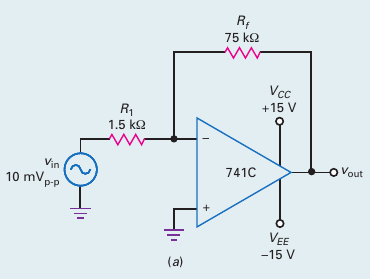
\includegraphics[width=\linewidth]{gambar/fig-16.17a}
		\end{center}
		\columnbreak
		\begin{itemize}
			\item Jawaban:
			\begin{itemize}
				\item Error tegangan input:
				\begin{align*}
					V_{1err} &= (R_{B1} - R_{B2})I_{in(bias)} \\
					&= ( - 1.47 \text{ k}\Omega )(500 \text{ nA}) \\
					&= -0.735 \text{ mV} \\
					V_{2err} &= (R_{B1} + R_{B2}) \frac{I_{in(off)}}{2} \\
					&= ( 1.47 \text{ k}\Omega )(100 \text{ nA}) \\
					&= 0.147 \text{ mV} \\
					V_{3err} &= V_{in(off)} = 6 \text{ mV}
				\end{align*}
			\end{itemize}
		\end{itemize}
	\end{multicols}
\end{frame}

\begin{frame}{Contoh Soal 2.9}
	\begin{multicols}{2}
		\begin{center}
			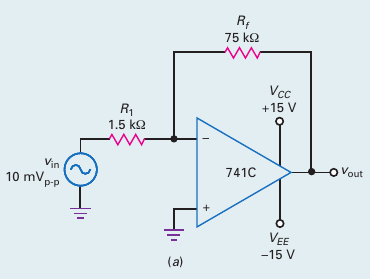
\includegraphics[width=\linewidth]{gambar/fig-16.17a}
		\end{center}
		\columnbreak
		\begin{itemize}
			\item Jawaban:
			\begin{itemize}
				\item Penguatan tegangan closed-loop:
				\[ A_{v(CL)} = \frac{-R_f}{R_1} = \frac{-75 \text{ k}\Omega}{1.5 \text{ k}\Omega} = -50\]
				\item Error tegangan output:
				\begin{align*}
					V_{error} &= \pm 50 (V_{1err} + V_{2err} + V_{2err}) \\
					&= \pm 50 (0.735 \text{mV} + 0.147 \text{mV} + 6 \text{mV}) \\
					&= \pm 344 \text{ mV}
				\end{align*}
			\end{itemize}
		\end{itemize}
	\end{multicols}
\end{frame}

\begin{frame}{Contoh Soal 2.9}
	\begin{figure}
		\centering
		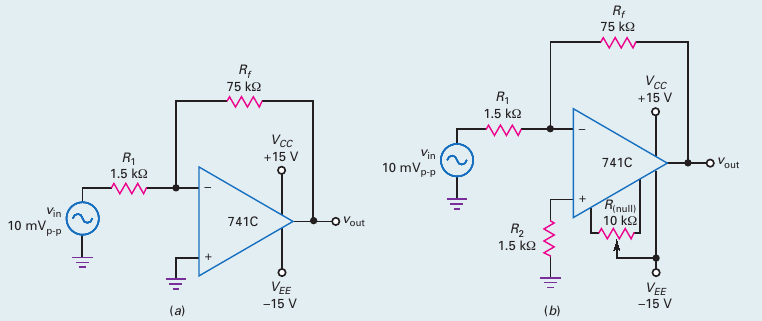
\includegraphics[width=0.8\linewidth]{gambar/fig-16.17}
		\caption{(a) Rangkaian op amp 741C dan (b) Rangkaian op amp 741C dengan penambahan compensating resistor dan potensiometer}
		\label{fig-16.17}
	\end{figure}
	
\end{frame}